\documentclass{a4beamer}
%% Lectures - common definitions

\usextensions{tikz}
\usetikzlibrary{shapes.multipart,shapes.callouts,shapes.geometric}
\input{fix-callouts.inc} % Fixes absolute positioning of rectangle callouts

\newif\ifbigpages \bigpagesfalse
\ifdim\paperwidth >20cm
	\bigpagestrue
\fi

\tikzset{%
	note/.style={rectangle callout,draw=none,callout pointer width=1em,%
		align=flush left,font=\footnotesize,inner sep=0.5em,%
		fill=blue!15,fill opacity=0.95,text opacity=1.0,callout absolute pointer=#1},
	node distance=2em and 2.75em
}
\ifbigpages
	% Scale all arrow tips by the factor of 2.5
	\let\old@pgf@arrow@call=\pgf@arrow@call
	\def\pgf@arrow@call#1{%
		\@tempdima=\pgflinewidth%
		\pgfsetlinewidth{2.5\pgflinewidth}%
		\old@pgf@arrow@call{#1}%
		\pgfsetlinewidth{\@tempdima}%
	}
	\def\pgfarrowsleftextend#1{\pgfmathsetlength{\pgf@xa}{1.5*#1}}
	\def\pgfarrowsrightextend#1{\pgfmathsetlength{\pgf@xb}{1.5*#1}}
\fi

%% Load listings package
\usepackage{listings}

%% Are we inside a comment?
\newif\iflstcomment \lstcommentfalse

\lstset{%
	tabsize=4,
	showstringspaces=false,
	basicstyle=\linespread{1.25}\ttfamily\small,
	keywordstyle=\bfseries,
	commentstyle=\lstcommentstyle,
	numbers=left,
	numberstyle=\footnotesize\color{gray},
	xleftmargin=2.5em,
	extendedchars=true,
	escapechar=\$,
	escapebegin=\iflstcomment\begingroup\lstcommentstyle\fi,
	escapeend=\iflstcomment\endgroup\fi
}

\def\lstcommentstyle{\color{gray}}

\lst@AddToHook{AfterBeginComment}{\global\lstcommenttrue}
\let\orig@lst@EndComment=\lst@EndComment
\def\lst@EndComment{\global\lstcommentfalse\orig@lst@EndComment}
\lst@AddToHookAtTop{EOL}{%
	\lst@ifLmode\global\lstcommentfalse\fi% XXX Sloppy way to determine comment end
}

%% Python with docstrings treated as comments
\lstdefinelanguage[doc]{python}[]{python}{%
	deletestring=[s]{"""}{"""},%
	morecomment=[s]{"""}{"""}%
}%

%% JavaScript language
\lstdefinelanguage{javascript}%
	{morekeywords={break,case,catch,%
		const,constructor,continue,default,do,else,false,%
		finally,for,function,if,in,instanceof,%
		new,null,prototype,%
		return,switch,this,throw,%
		true,try,typeof,var,while},%
	sensitive,%
	morecomment=[l]//,%
	morecomment=[s]{/*}{*/},%
	morestring=[b]",%
	morestring=[b]',%
}[keywords,comments,strings]%

%% C# language (4.0?)
\lstdefinelanguage{csharp}%
	{morekeywords={abstract,as,%
		base,bool,byte,case,catch,char,%
		checked,class,const,continue,%
		decimal,default,delegate,do,double,%
		else,enum,event,explicit,extern,%
		false,finally,fixed,float,for,foreach,%
		goto,if,implicit,in,int,interface,%
		internal,is,lock,long,%
		namespace,new,null,object,operator,out,%
		override,params,private,protected,public,%
		readonly,ref,return,sbyte,sealed,%
		short,sizeof,stackalloc,static,string,%
		struct,switch,this,throw,true,try,%
		typeof,uint,ulong,unchecked,unsafe,ushort,%
		using,virtual,void,volatile,while%
	},%
	sensitive,%
	morecomment=[l]//,%
	morecomment=[s]{/*}{*/},%
	morestring=[b]",%
	morestring=[b]',%
}[keywords,comments,strings]%

%% Translation for fact environment
\deftranslation[to=russian]{Fact}{Наблюдение}

%% Inline code snippets
\def\code#1{\texttt{#1}}
\def\codekw#1{\code{\textbf{#1}}}

\def\quoteauthor#1{\par\footnotesize\upshape\hfill—~#1}

%% English term
\def\engterm#1{(англ. \textit{#1})}
%% Term with explanation below (to be used in diagrams)
\def\termwithexpl#1#2{#1\strut{}\\\small\color{gray}(\textit{#2})\strut{}}
%% External link
\def\extlink#1#2{\href{#1}{\color[rgb]{0.7,0.7,1.0}\dashbar{#2}}}
%% Internal link
\def\inlink#1#2{\hyperlink{#1}{\color[rgb]{0.7,0.7,1.0}\dashbar{#2}}}
%% Explanation for a list item
\def\itemexpl#1{\begingroup\small\vspace{0.75ex}#1\par\endgroup}




\lecturetitle{Программная инженерия. Лекция №17 — Интерфейсы в программировании}
\title[Интерфейсы]{Интерфейсы в программировании}
\author{Алексей Островский}
\institute{\small{Физико-технический учебно-научный центр НАН Украины}\vspace{2ex}}
\date{2 апреля 2015 г.}

\begin{document}
	\frame{\titlepage}

	\section{Введение}

	\frame{
		\frametitle{Интерфейсы в программировании}

		\begin{Definition}
			\textbf{Интерфейс} — связь между двумя отдельными компонентами программной системы,
			предназначенная для обмена информацией, а также спецификация этой связи.
		\end{Definition}

		\vspace{1ex}
		\textbf{Виды интерфейсов:}
		\begin{itemize}
			\item аппаратные (в т.\,ч. для периферийных устройств);
			\item программные \engterm{software interfaces};
			\item пользовательские.
		\end{itemize}
		\textbf{NB.} Software interface $\supset$ (application) programming interface.

		\vspace{1ex}
		\textbf{Направленность} передачи данных:
		\begin{itemize}
		\item
			однонаправленные интерфейсы (напр., работа с мышью, микрофоном и другими устройствами);
			\item
			двунаправленные интерфейсы (напр., большинство программных).
		\end{itemize}
	}

	\subsection{Аппаратные интерфейсы}

	\frame{
		\frametitle{Аппаратные интерфейсы}

		\begin{figure}
			\ifbigpages
				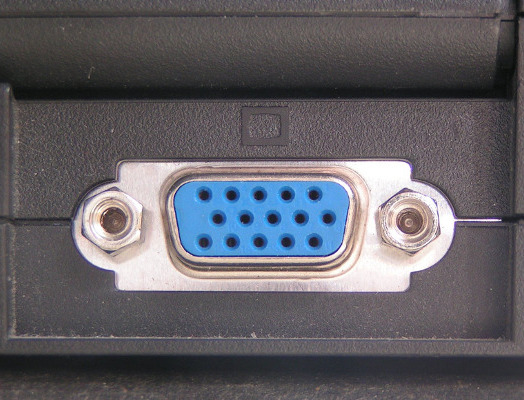
\includegraphics[scale=0.5]{fig-svga-port.jpg}
				\hspace{2em}
				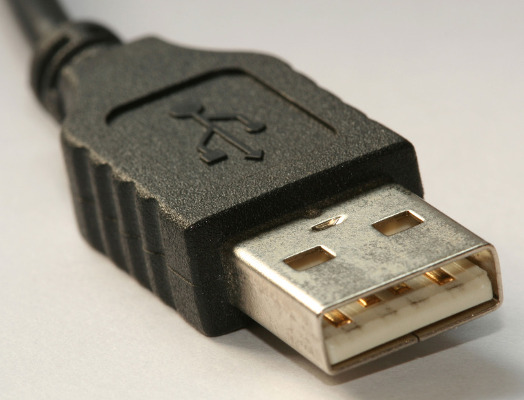
\includegraphics[scale=0.5]{fig-usb-connector.jpg}
			\else
				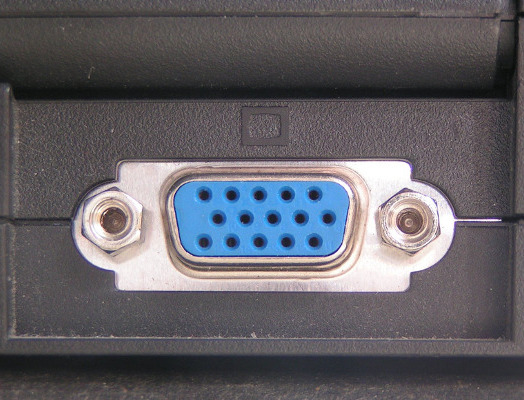
\includegraphics[scale=0.25]{fig-svga-port.jpg}
				\hspace{2em}
				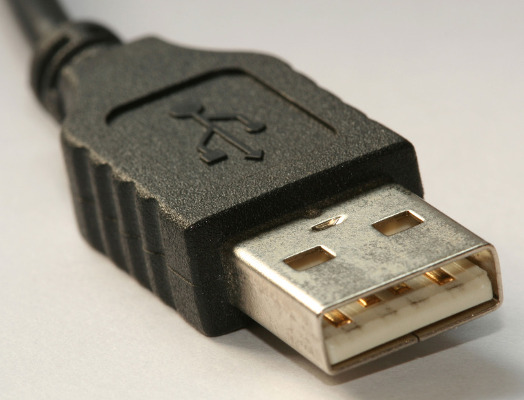
\includegraphics[scale=0.25]{fig-usb-connector.jpg}
			\fi
			\caption{Примеры аппаратных интерфейсов: %
				SVGA-вход для подключения видеоустройства и универсальная последовательная шина (USB).}
		\end{figure}
	}

	\frame{
		\frametitle{Аппаратные интерфейсы}

		\textbf{Виды:} шины, устройства хранения данных, радиоволны, …

		\vspace{1ex}
		\textbf{Спецификация:}
		\begin{itemize}
			\item характеристики механических, электрических или логических сигналов, пересылаемых через~интерфейс;
			\item последовательность передачи сигналов.
		\end{itemize}

		\vspace{1ex}
		\textbf{Цель:}
		\begin{itemize}
			\item унификация связи с базовыми и периферийными устройствами;
			\item большие возможности при конструировании и~сборке компьютерных систем.
		\end{itemize}
	}

	\subsection{Программные интерфейсы}

	\frame{
		\frametitle{Программные интерфейсы}

		\textbf{Уровень операционной системы:}
		\begin{itemize}
		\item связь программ с оборудованием (напр., с~помощью драйверов);
		\item связь программ с операционной системой или с~другими программами средствами~ОС.
		\end{itemize}

		\vspace{1ex}
		\textbf{Уровень приложения:}
		\begin{itemize}
		\item связь компонентов системы, написанных на разных ЯП,
		с помощью вспомогательной среды (middleware);
		\item связь компонентов распределенных приложений.
		\end{itemize}

		\vspace{1ex}
		\textbf{Уровень компонента:}\\
		связь между базовыми элементами программы (напр., между объектами в~ООП;
		между функциями в~функциональном программировании).
	}

	\frame{
		\frametitle{Уровень детализации интерфейса}

		\textbf{Двоичные интерфейсы} (ABI) — спецификации, связанные с \emph{машинным} кодом программной системы.

		\vspace{0.5ex}
		\textbf{Примеры:}
		\begin{itemize}
			\item размер в байтах типов данных;
			\item особенности вызовов функций / методов;
			\item формат двоичных исполняемых файлов.
		\end{itemize}

		\vspace{1.5ex}
		\textbf{Программные интерфейсы} (API) — спецификации, выражающиеся через \emph{исходный} код программы.

		\vspace{0.5ex}
		\textbf{Пример:}
		\begin{itemize}
			\item сигнатуры задекларированных функций / классов;
			\item протоколы обмена данными.
		\end{itemize}
	}

	\subsection{ABI}

	\frame{
		\frametitle{ABI}

		\begin{Definition}
			\textbf{Двоичный интерфейс приложений} \engterm{application binary interface, ABI}
			— программный интерфейс между двумя модулями (чаще всего, ОС~или~библиотекой и~прикладной программой),
			заданный на~уровне машинного кода.
		\end{Definition}

		\vspace{1ex}
		\textbf{Примеры спецификаций:}
		\begin{itemize}
			\item вызов функций (порядок аргументов, размещение аргументов в~стеке / регистрах);
			\item формат передачи данных (порядок передачи байтов, выравнивание);
			\item системные вызовы;
			\item формат исполняемых файлов, библиотек и~т.\,п.;
			\item обработка исключительных ситуаций.
		\end{itemize}
	}

	\frame{
		\frametitle{ABI}

		\textbf{Способы согласования ABI:}
			\begin{itemize}
			\item
			(в большинстве случаев) автоматически при компиляции / интерпретации программы;

			\vspace{1ex}
			\item
			при помощи специальных средств ЯП (напр., спецификаторы \code{safecall}, \code{stdcall} и~т.\,п.
			для~функций в~C/C++);

			\vspace{1ex}
			\item
			явно при использовании низкоуровневых средств взаимодействия между программами на~разных ЯП
			или при работе с~оборудованием (напр., чтение / запись данных в~память видеоускорителя).
		\end{itemize}
	}

	\frame{
		\frametitle{Примеры ABI}

		\begin{itemize}
			\item
			Спецификация \textbf{операционных систем}: Linux (\extlink{http://en.wikipedia.org/wiki/Linux_Standard_Base}{Linux Standard Base}),
			Windows, Mac~OS;

			\vspace{1ex}
			\item
			спецификация \textbf{виртуальных машин} и \textbf{сред выполнения}, напр., Java Virtual Machine:
			\begin{itemize}
				\item общая для всех имплементаций (напр., формат .class-файлов JVM);
				\item особенности имплементации в различных средах (напр., размеры указателей~JVM и~принципы сборки мусора).
			\end{itemize}

			\vspace{1ex}
			\item
			спецификация \textbf{языков программирования} (напр., размер, двоичное представление и~выравнивание типов данных);

			\vspace{1ex}
			\item
			EABI (embedded-application binary interface) — ABI для \textbf{встроенных} в~микропроцессор \textbf{программ}.
		\end{itemize}
	}

	\subsection{API}

	\frame{
		\frametitle{API}

		\begin{Definition}
			\textbf{Программный интерфейс приложений} \engterm{application programming interface, API}
			— спецификация утилит, протоколов и~инструментов для~интеграции компонентов приложений.
		\end{Definition}

		\vspace{1ex}
		\textbf{Примеры спецификаций:}
		\begin{itemize}
			\item
			характеристики компонентов повторного использования (операции, входные и~выходные данные);
			\item
			точки входа для расширения функциональности существующих приложений (плагины);
			\item
			программные «обертки» для доступа к оборудованию и~источникам данных (напр., СУБД).
		\end{itemize}
	}

	\frame{
		\frametitle{API}

		\textbf{Формы API:}
		\begin{itemize}
			\item
			Библиотека, содержащая функции / объекты, структуры данных, константы и~переменные.

			\vspace{0.5ex}
			\textbf{Примеры:} \extlink{http://en.wikipedia.org/wiki/Standard_Template_Library}{STL} для~С++; Java~API.

			\item
			Протокол для передачи данных.

			\vspace{0.5ex}
			\textbf{Примеры:} протоколы SOAP и REST для реализации веб-сервисов.
		\end{itemize}

		\vspace{1ex}
		\textbf{Формы спецификации:}
		\begin{itemize}
			\item международный стандарт (напр., \extlink{http://en.wikipedia.org/wiki/POSIX}{POSIX});
			\item документация производителя, независимая от ЯП + привязки к ЯП (напр., Windows~API, OpenGL);
			\item встроенная / подключаемая библиотека на определенном ЯП (STL, Java~APIs).
		\end{itemize}
	}

	\subsection{Сравнение API и ABI}

	\frame{
		\frametitle{Сравнение API и ABI}

		\textbf{API и ABI в C:}
		\lstinputlisting[language=c]{code-api-abi.c}
	}

	\frame{
		\frametitle{Сравнение API и ABI}

		\begin{itemize}
			\item
			GCC с опцией \code{-m32} (32-битный код для архитектуры i386):

			\vspace{0.5ex}
			\texttt{\small%
				sizeof(int) == 4\\%
				sizeof(long) == 4\\%
				sizeof(long double) == 12\\
				sizeof(void*) == 4\\%
			}

			\vspace{1ex}
			\item
			GCC с опцией \code{-mx32} (32-битный код для архитектуры x86\_64):

			\vspace{0.5ex}
			\texttt{\small%
				sizeof(int) == 4\\%
				sizeof(long) == 4\\%
				sizeof(long double) == 16\\%
				sizeof(void*) == 4\\%
			}

			\vspace{1ex}
			\item
			GCC с опцией \code{-m64} (64-битный код для архитектуры x86\_64):

			\vspace{0.5ex}
			\texttt{\small%
				sizeof(int) == 4\\%
				sizeof(long) == 8\\%
				sizeof(long double) == 16\\%
				sizeof(void*) == 8\\%
			}
		\end{itemize}
	}

	\section{Использование интерфейсов}

	\frame{
		\frametitle{Использование интерфейсов}

		\textbf{Варианты использования:}
		\begin{itemize}
			\item
			Интеграция компонентов, реализованных с помощью \emph{одного} ЯП.

			\vspace{1ex}
			\textbf{Реализация:}
			\begin{itemize}
				\item спецификация типов данных;
				\item контрактное программирование (напр., с помощью интерфейсов ЯП или утиной типизации);
				\item инверсия управления.
			\end{itemize}

			\item
			Интеграция компонентов, реализованных в \emph{разных} ЯП.

			\vspace{1ex}
			\textbf{Реализация:}
			\begin{itemize}
				\item использование общей исполняемой среды (виртуальной машины);
				\item вызов внешних функций;
				\item использование посредников (middleware).
			\end{itemize}
		\end{itemize}
	}

	\subsection{Интерфейсы ЯП}

	\frame{
		\frametitle{Пример: использование интерфейсов ЯП}

		\textbf{Процедурный подход}

		Интерфейсы ЯП определяются как спецификация структур данных и функций для~работы с~ними.

		\vspace{2ex}
		\textbf{Пример (C):}
		\lstinputlisting[language=c]{code-interfaces.c}
	}

	\frame{
		\frametitle{Пример: использование интерфейсов ЯП}

		\textbf{Объектно-ориентированный подход}

		Интерфейсы собраны в методах (конструкторах, свойствах и т.\,п.) объектов и~классов,
		содержащих в~себе данные и~зачастую скрывающих~их.

		\vspace{2ex}
		\textbf{Пример (Java)}
		\lstinputlisting[language=java]{code-interfaces.java}
	}

	\subsection{Инверсия управления}

	\frame{
		\frametitle{Инверсия управления}

		\begin{Definition}
			\textbf{Инверсия управления} \engterm{inversion of control} — принцип проектирования приложений,
			позволяющий передавать управление коду приложения во время выполнения сторонних библиотек.
		\end{Definition}

		\vspace{3ex}
		\begin{overlayarea}{\textwidth}{0.6\textheight}
			\only<1>{%
				\begin{figure}
					\begin{tikz*}[%
	every node/.style={rectangle,draw,align=center},
	big/.style={minimum width=10em,minimum height=7.5em},
	small/.style={minimum width=6em,minimum height=2.5em,fill=white},
	flow/.style={blue}
]
	\node(lib) [big] {Библиотека};
	\node(lib-func1) [above right=2em and 1em of lib.east,anchor=center,small] {\code{func1}};
	\node(lib-func2) [below right=2em and 1em of lib.east,anchor=center,small] {\code{func2}};

	\node(app) [big,right=15em of lib] {Приложение};
	\node(app-call1) [above left=2em and 1em of app.west,anchor=center,small] {\code{func1();}};
	\node(app-call2) [below left=2em and 1em of app.west,anchor=center,small] {\code{func2();}};

	\node(start) [coordinate, above=2em of app-call1.north] {};
	\node(finish) [coordinate, below=2em of app-call2.south] {};

	\draw[->,flow] (start)
		|- ($ (lib-func1.east) + (-0.5em, 0.75em) $)
		-- ++(0, -1.5em)
		-| (app-call1.south)
		|- ($ (lib-func2.east) + (-0.5em, 0.75em) $)
		-- ++(0, -1.5em)
		-| (app-call2.south)
		-- (finish);
\end{tikz*}

					\caption{\textbf{Традиционный подход} к работе с библиотеками.
						Библиотека определяет интерфейсы реализованных функций, которые вызываются приложением.
						{\color{blue}Синим} обозначен поток выполнения.}
				\end{figure}
			}
			\only<2>{%
				\begin{figure}
					\begin{tikz*}[%
	every node/.style={rectangle,draw,align=center},
	big/.style={minimum width=10em,minimum height=7.5em},
	small/.style={minimum width=6em,minimum height=2.5em,fill=white},
	flow/.style={blue}
]
	\node(lib) [big] {Библиотека};
	\node(lib-event1) [above right=2em and 1em of lib.east,anchor=center,small] {\code{event1}};
	\node(lib-event2) [below right=2em and 1em of lib.east,anchor=center,small] {\code{event2}};

	\node(app) [big,right=15em of lib] {Приложение};
	\node(app-handler1) [above left=2em and 1em of app.west,anchor=center,small] {\code{onEvent1}};
	\node(app-handler2) [below left=2em and 1em of app.west,anchor=center,small] {\code{onEvent2}};

	\node(start) [coordinate, above=2em of lib-event1.north] {};
	\node(finish) [coordinate, below=2em of lib-event2.south] {};

	\draw[->,flow] (start)
		|- ($ (app-handler1.west) + (0.5em, 0.75em) $)
		-- ++(0, -1.5em)
		-| (lib-event1.south)
		|- ($ (app-handler2.west) + (0.5em, 0.75em) $)
		-- ++(0, -1.5em)
		-| (lib-event2.south)
		-- (finish);
\end{tikz*}

					\caption{\textbf{Инверсия управления.}
						Основной код выполняется библиотекой; передача управления приложению происходит
						с~помощью точек расширения.}
				\end{figure}
			}
		\end{overlayarea}
	}

	\frame{
		\frametitle{Применение инверсии управления}

		\begin{itemize}
			\item
			\textbf{Обработка событий}, в частности при конструировании пользовательского интерфейса;

			\vspace{1ex}
			\item
			\textbf{расширение функциональности} приложений (плагины);

			\vspace{1ex}
			\item
			\textbf{упрощение построения} приложений на основе готовых каркасов (например, JavaBeans; аннотации в JUnit);

			\vspace{1ex}
			\item
			\textbf{наследование} в ООП, когда контроль выполнения задан в родительском классе
			(точки входа — абстрактные виртуальные методы).
		\end{itemize}
	}

	\frame{
		\frametitle{Пример: инверсия управления в DOM}

		Инверсия контроля — основной метод создания интерактивных HTML-документов
		с~помощью JavaScript.

		\vspace{1ex}
		\lstinputlisting[language=javascript]{code-dom.js}
	}

	\subsection{Виртуализация}

	\frame{
		\frametitle{Взаимодействие разноязыковых программ}

		\textbf{Методы взаимодействия} (по возрастанию усилий для реализации):
		\begin{itemize}
			\item
			вызов функций / методов в пределах одной среды выполнения (JVM, CLR);
			\item
			использование интерфейса внешних функций;
			\item
			использование распределенных систем (CORBA, RMI)\footnote{рассматриваются в~отдельной лекции.}
		\end{itemize}

		\vspace{1ex}
		\textbf{Проблемы} (следуют из различия ABI для разных ЯП):
		\begin{itemize}
			\item
			трансляция типов данных;
			\item
			различающиеся среды выполнения (напр., принципы сбора мусора);
			\item
			работа с разделяемой памятью.
		\end{itemize}
	}

	\frame{
		\frametitle{Виртуализация}

		\begin{Definition}
		\textbf{Виртуальная машина} \engterm{virtual machine} — программная среда
		для эмуляции вычислительной системы с~заданной конфигурацией и~интерфейсом.
		\end{Definition}

		\vspace{1ex}
		\textbf{Цели:}
		\begin{itemize}
		\item
			унификация доступных для программ интерфейсов в различных окружениях, улучшение переносимости;
			\item
			повышение отказоустойчивости и надежности;
			\item
			упрощение взаимодействия между программами в пределах ВМ;
			\item
			тестирование поведения ПО при заданной архитектуре или конфигурации оборудования.
		\end{itemize}
	}

	\frame{
		\frametitle{Спецификация ВМ}

		\begin{itemize}
			\item
			\textbf{Модель вычислений:} \extlink{http://en.wikipedia.org/wiki/Stack_machine}{стековая},
				\extlink{http://en.wikipedia.org/wiki/Register_machine}{регистровая};

			\vspace{1ex}
			\item
			\textbf{управление памятью:} автоматическое, вручную, смешанное, принцип работы сборщика мусора;

			\vspace{1ex}
			\item
			\textbf{метод выполнения кода:} интерпретация, \extlink{http://en.wikipedia.org/wiki/Just-in-time_compilation}{JIT}, компиляция);
			принципы комбинирования различных методов;

			\vspace{1ex}
			\item
			\textbf{взаимодействие модулей:} трансляция типов данных для различных ЯП,
			совместимость объектов в различных языках, работа с нативными библиотеками;

			\vspace{1ex}
			\item
			\textbf{безопасность:} возможность ограничений на выполняемые инструкции.
		\end{itemize}
	}

	\frame{
		\frametitle{Примеры ВМ}

		\begin{itemize}
			\item
			\textbf{Java Virtual Machine}

			\textbf{ЯП:} Java, Groovy, Scala, Clojure, Jython, JRuby, …

			\vspace{1ex}
			\item
			\textbf{Dalvik; Android Runtime (ART)}

			\textbf{ЯП:} поддерживаемые JVM (вход — байткод для JVM).

			\textbf{Примечание:} Dalvik / ART и JVM почти совместимы на уровне API,
			но используют разные ABI (регистровая машина в Dalvik / ART против стековой в JVM).

			\vspace{1ex}
			\item
			\textbf{Common Language Runtime; Mono}

			\textbf{ЯП:} C\#, F\#, Visual Basic .NET, IronPython, …

			\vspace{1ex}
			\item
			\textbf{LLVM} (Low Level Virtual Machine)

			\textbf{ЯП:} C, C++, D, Objective-C, Ada, Fortran.

			\textbf{Примечание:} часто используется в качестве компилятора.
		\end{itemize}
	}

	\frame{
		\frametitle{Пример ВМ: Java Virtual Machine}

		\begin{center}
			\begin{tikz*}[%
	every node/.style={rectangle,draw,align=center,minimum height=3.25em,minimum width=5em},
	cat/.style={font=\bfseries,draw=none}
]
	\node(loaders) [draw] {Загрузчики байткода \\ (напр., из файлов \textbf{*.class})};
	\node(class) [cat,left=of loaders] {Классы};

	\node(methods) [below=of loaders.south west,anchor=north west] {Методы};
	\node(heap) [right=1.5em of methods] {Куча};
	\node(stack) [right=1.5em of heap] {Стек JVM};
	\node(stack-native) [right=1.5em of stack] {Стек нативных \\ методов};
	\node(class) [cat,left=of methods] {Память};

	\node(interp) [below=of methods.south west,anchor=north west] {Интерпретатор};
	\node(jit) [right=1.5em of interp] {JIT-компилятор};
	\node(machine-code) [right=1.5em of jit] {Машинный код};
	\node(jni) [below=of interp.south west,anchor=north west] {Java Native Interface};
	\node(nat-libs) [right=1.5em of jni] {Нативные библиотеки};
	\node(exec) [cat,left=of interp] {Выполнение};

	\draw[->] (interp) -- (jit);
	\draw[->] (interp.south) -- (jni.north -| interp.south);
	\draw[->] (jit) -- (machine-code);
	\draw[->] (jni) -- (nat-libs);
\end{tikz*}

		\end{center}
	}

	\frame{
		\frametitle{Пример: взаимодействие программ в JVM}

		\begin{itemize}
			\item
			Языки, созданные \textbf{с~расчетом на~JVM} (Groovy, Scala) поддерживают импорт произвольных классов~Java
			(из~стандартной библиотеки и~сторонних).

			\vspace{1ex}
			\item
			Версии \textbf{адаптированных} для~JVM языков (Jython, JRuby) поддерживают классы~Java
			с~определенными предостережениями из-за~различия спецификаций.

			\vspace{1ex}
			\textbf{Пример.} Конфликты между Java и Jython:
			\begin{itemize}
				\item кодировки строк;
				\item области видимости;
				\item названия переменных и методов класса, совпадающие между~собой
				или~с~ключевыми словами Python.
			\end{itemize}

			\vspace{1ex}
			\item
			Использование языков JVM \textbf{из~Java} возможно за~счет увеличения сложности структуры программ
			(напр., применение
			\extlink{http://www.jython.org/jythonbook/en/1.0/JythonAndJavaIntegration.html}{фабрик объектов}
			или \extlink{http://docs.oracle.com/javase/7/docs/technotes/guides/scripting/programmer_guide/}{Java Scripting API}
			для~Jython).
		\end{itemize}
	}

	\subsection{Интерфейс внешних функций}

	\frame{
		\frametitle{Интерфейс внешних функций}

		\begin{Definition}
			\textbf{Интерфейс внешних функций} \engterm{foreign function interface} — механизм поддержки вызова программой,
			написанной на~одном~ЯП, функций, реализованных на~других~ЯП.
		\end{Definition}

		\vspace{1ex}
		\textbf{Цели:}
		\begin{itemize}
			\item повышение производительности;
			\item вызов специфичных для платформы функций.
		\end{itemize}

		\vspace{1.5ex}
		\begin{figure}
			\begin{tikz*}[%
	every node/.style={rectangle,draw,align=center,minimum height=3.5em,minimum width=8.5em},
	label/.style={minimum height=0pt,minimum width=0pt,font=\small,draw=none}
]
	\node(hi-level) {Программа на \\ высокоуровневом \\ ЯП};
	\node(ffi-lib) [right=5em of hi-level] {Библиотека \\ FFI};
	\node(lo-level) [right=5em of ffi-lib] {Программа на \\ низкоуровневом \\ ЯП (C, C++, ASM)};

	\draw[->] (hi-level) -- node[above,label]{API} (ffi-lib);
	\draw[->] (ffi-lib) -- node[above,label]{ABI} (lo-level);
\end{tikz*}

			\caption{Типичная архитектура интерфейса внешних функций}
		\end{figure}
	}

	\frame{
		\frametitle{Примеры FFI}

		\begin{itemize}
			\item
			Директивы \code{\codekw{extern} "C"} в С++ для вызова C-функций.

			\vspace{1ex}
			\item
			Java Native Interface, Java Native Access.

			\vspace{1ex}
			\item
			Модуль \code{ctypes} в Python для вызова функций C:

			\vspace{1ex}
			\lstinputlisting[language=python]{code-ffi.py}
		\end{itemize}
	}

	\section{Заключение}

	\subsection{Выводы}

	\frame{
		\frametitle{Выводы}

		\begin{enumerate}
			\item
			Интерфейсы — необходимая часть системы, составленной из разнородных компонентов.
			Интерфейс определяет способ обмена данными между компонентами программной системы.

			\vspace{0.5ex}
			\item
			Выделяют два типа программных интерфейсов: определяющие характеристики данных
			на~уровне машинного кода (ABI) и~на~уровне языков программирования (API).

			\vspace{0.5ex}
			\item
			Интерфейсы применяются для связи компонентов в~пределах одного~ЯП
			(за~счет спецификации типов данных, протоколов работы с~ними, инверсии управления и~т.\,д.)
			или~для~связи разноязычных компонентов.

			\vspace{0.5ex}
			\item
			Основные способы взаимодействия~ЯП: общая среда выполнения (виртуальная машина);
			интерфейсы внешних функций; протоколы передачи данных с~помощью посредников.
		\end{enumerate}
	}

	\subsection{Материалы}

	\frame{
		\frametitle{Материалы}

		\begin{thebibliography}{9}
			\bibitem[1]{1}
			Лавріщева К.\,М.
			\newblock Програмна інженерія (підручник).
			\newblock {\footnotesize К., 2008. — 319 с.}

			\bibitem[2]{2}
			Bloch, Joshua
			\newblock Руководство по написанию API.
			\newblock {\footnotesize \url{http://lcsd05.cs.tamu.edu/slides/keynote.pdf}}

			\bibitem[3]{3}
			Fowler, Martin
			\newblock Inversion of Control
			\newblock {\footnotesize \url{http://martinfowler.com/bliki/InversionOfControl.html}}
		\end{thebibliography}
	}

	\frame{
		\frametitle{}

		\begin{center}
			\Huge Спасибо за внимание!
		\end{center}
	}
\end{document}
